\documentclass[a4paper,12pt]{article}


\usepackage{ProfModels}
\usepackage{amssymb}
\usepackage{graphicx}
 \newcommand{\nonparallel}{\mathbin{\rotatebox[origin=c]{-90\shortmid}{$\nparallel$}}}
\begin{document}

\begin{Maquette}[Fiche]{Theme=Notions de géométrie,Niveau=1}

\begin{exercice}
Observe la figure et rependre aux questions par "parallèles" ; "sécantes" ; "confondus".
\begin{tasks}(3)
\task $\lrp{D}$ et $\lrp{K}$ sont :
\task $\lrp{K}$ et $\lrp{AB}$ sont :
\task $\lrp{D}$ et $\lrp{EB}$ sont :
\task $\lrp{EB}$ et $\lrp{AF}$ sont :
\task $\lrp{D}$ et $\lrp{EA}$ sont :
\task $\lrp{K}$ et $\lrp{FB}$ sont :
\task $\lrp{EF}$ et $\lrp{D}$ sont :
\task $\lrp{AF}$ et $\lrp{EB}$ sont :
\task $\lrp{D}$ et $\lrp{BF}$ sont :
\end{tasks}
\begin{tikzpicture}[scale=0.8]
\tkzDefPoints{0/0/E,4/0/F,-1/-2/B,5/-2/A}
\tkzDrawLines(E,F A,B E,A E,B F,A)
\tkzLabelPoints[above](E,F)
\tkzLabelPoints(A,B)
\tkzLabelLine[pos=1.2,left](F,E){$(D)$}
\tkzLabelLine[pos=1.2,below](A,B){$(K)$}
\end{tikzpicture}
\end{exercice}

\begin{exercice}
Compléter par le symbole $\in$ ou $\notin$.
\begin{tasks}(4)
\task $A \cdots (BM) $
\task $K \cdots (D) $
\task $D \cdots [BM] $
\task $R \cdots (GK) $
\task $C \cdots [RN) $
\task $P \cdots (RN) $
\task $P \cdots [RN] $
\task $D \cdots [AM] $
\task $G \cdots (\Delta) $
\task $N \cdots [AR) $
\task $A \cdots [NC) $
\task $A \cdots [BD) $
\task $M \cdots (\Delta) $
\task $R \cdots (AG) $
\task $M \cdots [KD) $
\task $P \cdots (GD) $
\end{tasks}
\begin{tikzpicture}
\tkzDefPoints{0/0/A,3/1/B,2/-1/C,0/1/G}
\tkzDefPointOnLine[pos=0.4](A,B)\tkzGetPoint{D}
\tkzDefPointOnLine[pos=1.3](A,B)\tkzGetPoint{M}
\tkzDefPointOnLine[pos=-0.4](A,B)\tkzGetPoint{K}
\tkzDefPointOnLine[pos=0.4](A,C)\tkzGetPoint{N}
\tkzDefPointOnLine[pos=0.8](A,C)\tkzGetPoint{P}
\tkzDefPointOnLine[pos=-0.4](A,C)\tkzGetPoint{R}
\tkzDrawPoints(A,B,C,G,D,M,K,N,P,R)
\tkzDrawLines(M,K R,C G,R)
\tkzLabelLine[pos=1.2,left](M,K){$(D)$}
\tkzLabelLine[pos=1.2,left](C,R){$(\Delta)$}

\tkzLabelPoints(A,B,C,G,D,M,K,N,P,R)
\end{tikzpicture}
\end{exercice}

\begin{exercice}
\begin{enumerate}
\item Trace une droite $(D)$ et un point $A$ qui l'appartient.
\item Trace un point $B$ qui n'appartient pas à $(D)$.
\item Trace la droite qui passe par $B$ et coupe $(D)$ en $A$.
\item Trace la droite  parallèle à $(D)$ et qui passe par $B$.
\end{enumerate}
\end{exercice}

\begin{exercice}
Soit $(\Delta)$ une droite , $A$ et $B$ deux points qui n'appartiennent pas à $(\Delta)$.
\begin{enumerate}
\item Trace $O$ le milieu de $\lrc{AB}$.
\item Trace $E$ le projeté orthogonal de $A$ sur $(\Delta)$.
\item Trace $F$ le projeté orthogonal de $B$ sur $(\Delta)$.
\item Trace $M$ le projeté orthogonal de $O$ sur $(\Delta)$.
\end{enumerate}
\end{exercice}

\begin{exercice}
Trace quatre points alignés $A$, $B$, $C$ et $D$ dans chaque cas:
\begin{enumerate}
\item $A\in [DC)$ et $C\in [AB]$.
\item $D\in [BC]$ et $C\in [AB)$.
\item $D$ milieu de $[AC]$ et $B\in [AD]$ et $B\in [AD]$.
\end{enumerate}
\end{exercice}

\begin{exercice}
Soit $A$, $B$ et $C$ trois points non alignés.
\begin{enumerate}
\item Trace trois droites $(D)$ et $(L)$ et $(K)$ sachant que :
\begin{enumerate}
\item $(D)$ passe par $A$ et $B$.
\item $(L)$ parallèle à $(D)$ et passe par $C$.
\item $(K)$ coupe  $(D)$ en $A$ et  $(L)$ en $C$.
\end{enumerate}
\end{enumerate}
\end{exercice}

\begin{exercice}
\begin{minipage}{0.6\linewidth}
On considère la figure ci-contre 
\begin{enumerate}
\item Trace une droite $(\Delta)$ parallèle à $(D)$ et passe par $A$
\item Trace $E$ le projeté orthogonal de $C$ sur $(D)$
\item Trace $F$ le milieu de $\lrc{AC}$
\item Trace la droite perpendiculaire à $(AC)$ en $F$.
\end{enumerate}
\end{minipage}%
\begin{minipage}{0.4\linewidth}
\begin{tikzpicture}
\tkzDefPoints{0/0/B,3/2/A,2/-1/C}
\tkzDrawPoints(A,B,C)
\tkzDrawLine[add=0.2 and 0.1](A,B)
\tkzLabelPoints(A,B,C)
\tkzLabelLine[pos=1.1,left](A,B){$(D)$}
\end{tikzpicture}
\end{minipage}
\end{exercice}

\begin{exercice}
\begin{minipage}{0.7\linewidth}
\begin{enumerate}
\item Reproduire la figure ci-contre.
\item Construire $\lrp{\Delta}$ la droite perpendiculaire à $\lrp{D}$ passant par $A$.
\item Constuire  $\lrp{\Delta '}$ la droite perpendiculaire à $\lrp{D}$ passant par $B$. 
\item Quelle est la position relative des droites $\lrp{\Delta}$ et $\lrp{\Delta '}$?
\end{enumerate}
\end{minipage}\vline%
\begin{minipage}{0.3\linewidth}
\begin{tikzpicture}
\tkzDefPoints{0/0/B,2/-0.3/C,2/1/A}
\tkzDrawLine[add=0.2 and 0.2](B,C)
\tkzDrawPoint(A)
\tkzLabelLine[pos=1.2,left](C,B){$(D)$}
\tkzLabelPoint[left](A){A}
\end{tikzpicture}
\end{minipage}
\end{exercice}

\begin{exercice}
\begin{enumerate}
\item Placer sur une droite $\lrp{D}$ deux points $A$ et $B$ tels que $AB=4$.
\item Construire une droite $\lrp{D1}$ parallèle à $\lrp{D}$.
\item Construire $\lrp{D2}$ la perpendiculaire au support de $\lrc{AB}$ en son milieu.
\item Montrer que $\lrp{D1}$ et $\lrp{D2}$ sont perpendiculaires.
\end{enumerate}
\end{exercice}

\begin{exercice}
\begin{enumerate}
\item Construire deux droitres $\lrp{D1}$ et $\lrp{D2}$ perpendiculaires en $A$.
\item Marquer un point $B$ distinct de $A$ sur $\lrp{D1}$.
\item Tracer la droite $\lrp{D3}$ passant par $B$ et perpendiculaire à $\lrp{D1}$.
\item Donner la position relative des droites $\lrp{D1}$ et $\lrp{D3}$.
\item Marquer un point $C$ distinct de $B$ sur $\lrp{D3}$.
\item Tracer la droite $\lrp{D4}$ passant par $C$ et perpendiculaire à $\lrp{D3}$.
\item Donner la position relative des droites $\lrp{D1}$ et $\lrp{D4}$.
\item Marquer un point $E$ intersection des droites $\lrp{D4}$ et $\lrp{D2}$.
\item La droite $\lrp{D4}$ est-elle perpendiculaire à $\lrp{D2}$?
\end{enumerate}
\end{exercice}








\end{Maquette}
\end{document}